\setmodule{9}

%BEGIN_FOLD % ====>>_____ Занятие 1 _____<<====
\begin{class}[number=1-2]
	\title{Занятие 1}
	\begin{definit}
		Координатная прямая --- это прямая, имеющая направление, начало отсчета и заданный масштаб.
	\end{definit}
	\begin{minipage}[c]{0.9\linewidth}
		\includegraphics[align=t, width=\linewidth]{\picpath/../../bank/graphs/graph_gleb/7/straight}
	\end{minipage}
	\begin{definit}
		Координатная плоскость --- это прямоугольная система координат, состоящая из двух взаимно перпендикулярных осей, имеющих направление, начало отсчета и единичные отрезки.
	\end{definit}
	\begin{definit}
		Начало координат --- точка \(O\).
		Оси координат --- прямые \(x\) и \(y\).
	\end{definit}
	\begin{minipage}[c]{0.5\linewidth}
		\includegraphics[align=t, width=\linewidth]{\picpath/../../bank/graphs/graph_gleb/7/coord}
	\end{minipage}\\
	\begin{minipage}[c]{0.6\linewidth}
		\begin{definit}
			Строгий знак означает, что точка \textbf{не} включается в промежуток: \(x>a\). \\
			Нестрогий знак означает, что точка включается в промежуток: \(x\ge b\).
		\end{definit}
	\end{minipage}
	\begin{minipage}[c]{0.4\linewidth}
		\includegraphics[align=t, width=\linewidth]{\picpath/../../bank/graphs/graph_gleb/7/points}
	\end{minipage}
	\begin{listofex}
		\item Отметьте на координатной прямой точки, удовлетворяющие неравенству. Запишите какие-нибудь три числа, удовлетворяющие этому неравенству и, если возможно, наибольшее и наименьшее целое число, удовлетворяющие этому неравенству.
		\begin{tasks}(3)
			\task \( x \le 5 \)
			\task \( x \le 2 \)
			\task \( x < 4 \)
			\task \( z<3 \)
			%\task \( x \ge 6 \)
			\task \( x \ge 1 \)
			%\task \( x > -5 \)
			\task \( x > -2 \)
			%\task \( -2 \le x \le 5 \)
			\task \( -5 \le x \le 1 \)
			\task \( -2 < x < 7 \)
			\task \( -3 < x < 4 \)
			\task \( -1 \le x \le 4 \)
			\task \( -4 < x \le 1 \)
			\task \( 3 \le x < 6 \)
			%\task \( -1 < x \le 8 \)
		\end{tasks}
		\item Отметьте на координатной прямой точки, удовлетворяющие системе неравенств. Запишите какие-нибудь три числа, удовлетворяющие этой системе неравенств и, если возможно, наибольшее и наименьшее целое число, удовлетворяющие этой системе неравенств.
		\begin{tasks}(4)
			\task \( \begin{cases} x \ge 5 \\ x \le 7 \end{cases} \)
			\task \( \begin{cases} x \ge 1 \\ x \le 5 \end{cases} \)
			\task \( \begin{cases} x>5 \\ x<6 \end{cases} \)
			\task \( \begin{cases} x<7 \\ x>5 \end{cases} \)
			%\task \( \begin{cases} x > -3 \\ x < 0 \end{cases} \)
			\task \( \begin{cases} x>0 \\ x<3 \end{cases} \)
			\task \( \begin{cases} x\le5 \\ x>1 \end{cases} \)
			\task \( \begin{cases} x<-1 \\ x\ge-4 \end{cases} \)
			\task \( \begin{cases} x<4 \\ x\ge3 \end{cases} \)
			%\task \( \begin{cases} x\ge4 \\ x>4 \end{cases} \)
		\end{tasks}
		\item Отметьте на координатной прямой точки, удовлетворяющие совокупности неравенств. Запишите какие-нибудь три числа, удовлетворяющие этой совокупности неравенств и, если возможно, наибольшее и наименьшее целое число, удовлетворяющие этой совокупности неравенств.
		\begin{tasks}(2)
			\task \( \left[ 
			\begin{array}{l}
				x>-2\\
				x>6
			\end{array}
			\right. \)
			\task \( \left[
			\begin{array}{l} x<1 \\ x<-3 \end{array} \right. \)
			\task \( \left[
			\begin{array}{l} x \le -4 \\ x>-1 \end{array} \right. \)
			\task \( \left[
			\begin{array}{l} x \le -2 \\ x < -5 \end{array} \right. \)
			\task \( \left[
			\begin{array}{l} -2 \le x \le 0 \\ -4 < x < -1 \end{array} \right. \)
			%\task \( \left[
			%\begin{array}{l} 0<x \le 7 \\ -4 < x < 9 \end{array} \right. \)
			\task \( \left[
			\begin{array}{l} -2 \le x \le 0 \\ -4<x<-1 \end{array} \right. \)
			%\task \( \left[
			%\begin{array}{l} 0<x \le 7 \\ -4<x<-1 \end{array} \right. \)
		\end{tasks}
	\end{listofex}
	\title{Занятие 2}
	\begin{listofex}[resume]
		%c190 n6.1 VES
		%n6.2 д-й
		%6.4 a-g
		%6.5
		\item
		\begin{minipage}[c]{0.6\linewidth}
			На рисунке изображены точки \( A (2;3) \), \( B(0;4) \), \( C(3;0) \), \( D(-4;-2) \). Назовите абсциссу и ординату каждой точки. Запишите координаты точек \( M \), \( N \), \( K \), \( L \). В каких координатных углах расположены точки \( A \), \( D \), \( L \), \( K \)?
		\end{minipage}
		\begin{minipage}[c]{0.4\linewidth}
			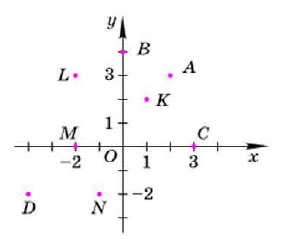
\includegraphics[align=t, width=\linewidth]{\picpath/G61M9L1}
		\end{minipage}
		\item Постройте систему координат и отметьте точки
		\begin{tasks}(4)
			\task \( A(4;3) \)
			\task \( B(2;4) \)
			\task \( C(-5;2) \)
			\task \( D(4;-3) \)
			\task \( E(-5;-1) \)
			\task \( M(1;3) \)
			\task \( N(3;0) \)
			\task \( K(0;4) \)
		\end{tasks}
		\item Отметьте на координатной прямой точки, удовлетворяющие условию:
		\begin{tasks}(5)
			\task \( |x|=4 \)
			\task \( |x|=1 \)
			\task \( |x|=7 \)
			\task \( |x|=2 \)
			\task \( |x|=0 \)
		\end{tasks}
		\item Известно, что \( |a|<|b| \). Как могут быть расположены на числовой прямой числа \( a \) и \( b \). Перечислите все возможные случаи. Схематично изобразите все случаи на числовой прямой.
		\item Известно, что \( |a|<|b|<|c| \). Как могут быть расположены на числовой прямой числа \(a, b\) и \(c\). Перечислите все возможные случаи. Схематично изобразите все случаи на числовой прямой.
		\item Постройте фигуру животного по точкам: \( (4;-3) \), \( (2;-3) \), \( (2;-2) \), \( (4;-2) \), \( (4;-1) \), \( (3;1) \), \( (2;1) \), \( (1;2) \), \( (0;0) \), \( (-3;2) \), \( (-4;5) \), \( (0;8) \), \( (2;7) \), \( (6;7) \), \( (8;8) \), \( (10;6) \), \( (10;2) \), \( (7;0) \), \( (6;2) \) \( (6;-2) \), \( (5;-3) \), \( (4;-3) \), \( (4;-5) \), \( (3;-9) \), \( (0;-8) \), \( (1;-5) \), \( (1;-4) \), \( (0;-4) \), \( (0;-9) \), \( (-3;-9) \), \( (-3;-3) \), \( (-7;-3) \), \( (-7;-7) \),  \( (-8;-7) \), \( (-8;-8) \), \( (-11;-8) \), \( (-10;-4) \), \( (-11;-1) \), \( (-14;-3) \), \( (-12;-1) \), \( (-11;2) \), \( (-8;4) \), \( (-4;5) \). Постройте отдельно две точки: \( (2;4) \), \( (6;4) \) --- это глаза животного.
	\end{listofex}
\end{class}
%END_FOLD

%BEGIN_FOLD % ====>>_ Домашняя работа 1 _<<====
\begin{homework}[number=1]
	\begin{listofex}
	%c190 n6.1 VES
	\item Отметьте на координатной прямой точки, удовлетворяющие неравенству. Запишите какие-нибудь три числа, удовлетворяющие этому неравенству и, если возможно, наибольшее и наименьшее целое число, удовлетворяющие этому неравенству.
	\begin{tasks}(2)
		%\task \( x \le -7,5 \)
		\task \( x \ge \dfrac{ 1 }{ 3 } \)
		\task \( x > 1 \)
		%	\task \( x > -9 \)
		%\task \( 2,5 \le x \le 4,1 \)
		\task \( -5 < x \le 0 \)
		%\task \( 0 \le x < 2 \)
		\task \( -1 < x \le 0,5 \)
	\end{tasks}
	
	
	%6.4 a-g
	\item Отметьте на координатной прямой точки, удовлетворяющие совокупности неравенств. Запишите какие-нибудь три числа, удовлетворяющие этой совокупности неравенств и, если возможно, наибольшее и наименьшее целое число, удовлетворяющие этой совокупности неравенств.
	\begin{tasks}(2)
		\task \( \left[
		\begin{array}{l} 5 \le x \le 8 \\ 2 < x < 7 \end{array} \right. \)
		\task \( \left[
		\begin{array}{l} -2<x \le 5 \\ -11 < x < 2 \end{array} \right. \)
	\end{tasks}
	%n6.2 д-й
	\item Отметьте на координатной прямой точки, удовлетворяющие системе неравенств. Запишите какие-нибудь три числа, удовлетворяющие этой системе неравенств и, если возможно, наибольшее и наименьшее целое число, удовлетворяющие этой системе неравенств: \[ \begin{cases} x > -1 \\ x < 5 \end{cases} \]
	%\begin{tasks}(3)
	%	\task 
	%	\task \( \begin{cases} x<4 \\ x>3 \end{cases} \)
	%	\task \( \begin{cases} -2 \le x < 5 \\ -1 < x < 8 \end{cases} \)
	%\end{tasks}
	%\item Известно, что \( |a|\ge |b| \). Как могут быть расположены на числовой прямой числа \( a \) и \( b \). Перечислите все возможные случаи. Схематично изобразите все случаи на числовой прямой.
	%6.5
	\item Отметьте на координатной прямой точки, удовлетворяющие условию:
	\begin{tasks}(4)
		\task \( |x|=1 \)
		\task \( |x|=3 \)
		\task \( |x|=5 \)
		\task \( |x|=11 \)
	\end{tasks}
	\item Постройте систему координат и отметьте точки
	\begin{tasks}(4)
		\task \( A(1;6) \)
		\task \( B(4;4) \)
		\task \( C(-2;-5) \)
		\task \( D(7;-3) \)
		\task \( E(-4;2) \)
		\task \( M(5;8) \)
		\task \( N(3;-6) \)
		\task \( K(-2;-4) \)
	\end{tasks}
	\end{listofex}
\end{homework}
%END_FOLD

%BEGIN_FOLD % ====>>_____ Занятие 3 _____<<====
\begin{class}[number=3]
	\begin{listofex}
		\item Занятие 3 
	\end{listofex}
\end{class}
%END_FOLD

%BEGIN_FOLD % ====>>_____ Занятие 4 _____<<====
\begin{class}[number=4]
	\begin{listofex}
		\item Занятие 4
	\end{listofex}
\end{class}
%END_FOLD

%BEGIN_FOLD % ====>>_ Домашняя работа 2 _<<====
\begin{homework}[number=2]
	\begin{listofex}
		\item Домашняя работа 2
	\end{listofex}
\end{homework}
%END_FOLD

%BEGIN_FOLD % ====>>_____ Занятие 5 _____<<====
\begin{class}[number=5]
	\begin{listofex}
		\item Занятие 5
	\end{listofex}
\end{class}
%END_FOLD

%BEGIN_FOLD % ====>>_____ Занятие 6 _____<<====
\begin{class}[number=6]
	\begin{listofex}
		\item Занятие 6
	\end{listofex}
\end{class}
%END_FOLD

%BEGIN_FOLD % ====>>_ Домашняя работа 3 _<<====
\begin{homework}[number=3]
	\begin{listofex}
		\item Домашняя работа 3
	\end{listofex}
\end{homework}
%END_FOLD

%BEGIN_FOLD % ====>>_____ Занятие 7 _____<<====
\begin{class}[number=7]
	\title{Подготовка к проверочной}
	\begin{listofex}
		\item Занятие 7
	\end{listofex}
\end{class}
%END_FOLD

%BEGIN_FOLD % ====>>_ Проверочная работа _<<====
\begin{exam}
	\begin{listofex}
		\item Проверочная
	\end{listofex}
\end{exam}
%END_FOLD